\documentclass{article}

%Hỗ trợ gõ tiếng việt
\usepackage[utf8]{inputenc}
\usepackage[vietnam]{babel}

\usepackage{graphicx}
\usepackage{hyperref}

%\usepackage[all]{hypcap} %Chỉnh tham chiếu chéo lên phía trên caption

%Thử câu lệnh sau:
%\renewcommand{\figurename}{Hinh}

\begin{document}

%YÊU CẦU 1: Tạo danh sách hình ảnh và bảng biểu
%\listoffigures
\listoftables

\section{Chú thích ảnh}
\label{section:figure} %Gánh nhãn cho phần này
Viết cái gì đó\ldots\\

\begin{figure}[h] % Thử thay đổi các giá trị sau \h \t \b \h!...
\center
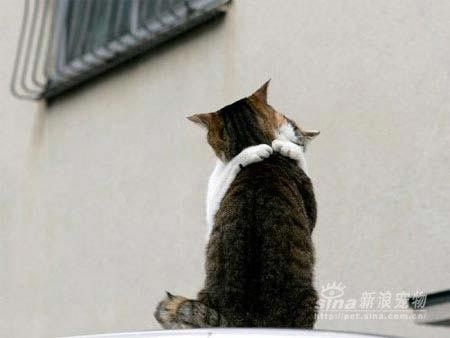
\includegraphics[scale=0.3]{meo}
\caption[Đây là dòng chú thích rút gọn cho ảnh 1]{Đây là dòng chú thích đầy đủ cho ảnh trên. 2 con mèo đang vật lộn với nhau.}
\label{figure:cat}
\end{figure}
%YÊU CẦU 2: Thử bỏ đoạn chú thích trong dấu [....] và biên dịch lại xem List of Figures thay đổi như thế nào
\begin{figure}[h]
\center
\caption[Đây là dòng chú thích rút gọn cho ảnh 2]{Đây là dòng chú thích đầy đủ cho ảnh nhưng nằm phía trên ảnh. Ảnh 2 con mèo đang vật lộn với nhau nhưng bị đảo ngược lại.}
\label{figure:cat_reversed}
\hfill\\
\reflectbox{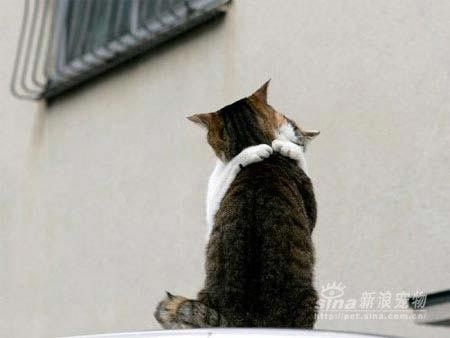
\includegraphics[scale=0.3]{meo}}
\end{figure}

\section{Chú thích bảng biểu}
%------TABLE------\\[0.5cm]
\label{section:table}
\begin{table}[h]
\center
  \begin{tabular}{| c | c |}
	\hline
	a & b \\ \hline
	c & d \\
	\hline
  \end{tabular}
\caption{Đây là dòng chú thích cho bảng.}
\label{table:abcd}
\end{table}
%\label{table:abcd} %Thử xóa dòng trên và thay bằng dòng này

\hfill\\

\section{Tham chiếu chéo}

\hfill\\
\phantomsection %dùng tham chiếu đến vị trí bất kì
\label{thử_nghiệm1}
Ta có thể tham chiếu đến một vị trí bất kì.
\hfill\\
%YÊU CẦU 3: Thêm tham chiếu đến trang
Đây là một tham chiếu chéo đến ảnh \ref{figure:cat} ở trang \\
%YÊU CẦU 4: Thêm tham chiếu đến ảnh
Đây là một tham chiếu chéo đến ảnh 2 ở trang \pageref{figure:cat_reversed}\\
2 ảnh này nằm trong phần \ref{section:figure}

\hfill\\
Đây là một tham chiếu chéo đến bảng \ref{table:abcd} ở trang \pageref{table:abcd}\\
%YÊU CẦU 5: Gán nhãn đến phần Chú thích ảnh
Bảng này nằm trong phần ...

\begin{equation} \label{equation:example}
x^2 - 5 x + 6 = 0
\end{equation}
Đây là một tham chiếu đến phương trình (\ref{equation:example}) %Thường công thức, phương trình, ... hay viết trong dấu ngoặc

Còn đây là tham chiếu đến vị trí bất kì \ref{thử_nghiệm1}

\end{document}
